\subsection{Data Deletion - Susmit} \label{sec:data-delete}


\subsubsection{Scenario} 
The same Alice found in Subsection~\ref{sec:data-insert} finds out that she made a grave mistake in pre-processing (i.e. indexing) the axolotl genome three weeks after she had inserted the data into Hydra. While Alice can wait a few more weeks to let the data naturally remove itself due to Hydra's base policy, she fears that anyone using her data before it gets removed will get false hope and possibly base future research on false data. This is a major concern for Clemson's Genomics and Bioinformatics facility as it can harmfully affect the facility's goal with using Hydra. Therefore, Alice needs a way to delete a file. To satisfy this scenario, the following interactions are conducted.


\subsubsection{User-to-Node Interaction} 
\begin{figure}[!ht]
    \centering
    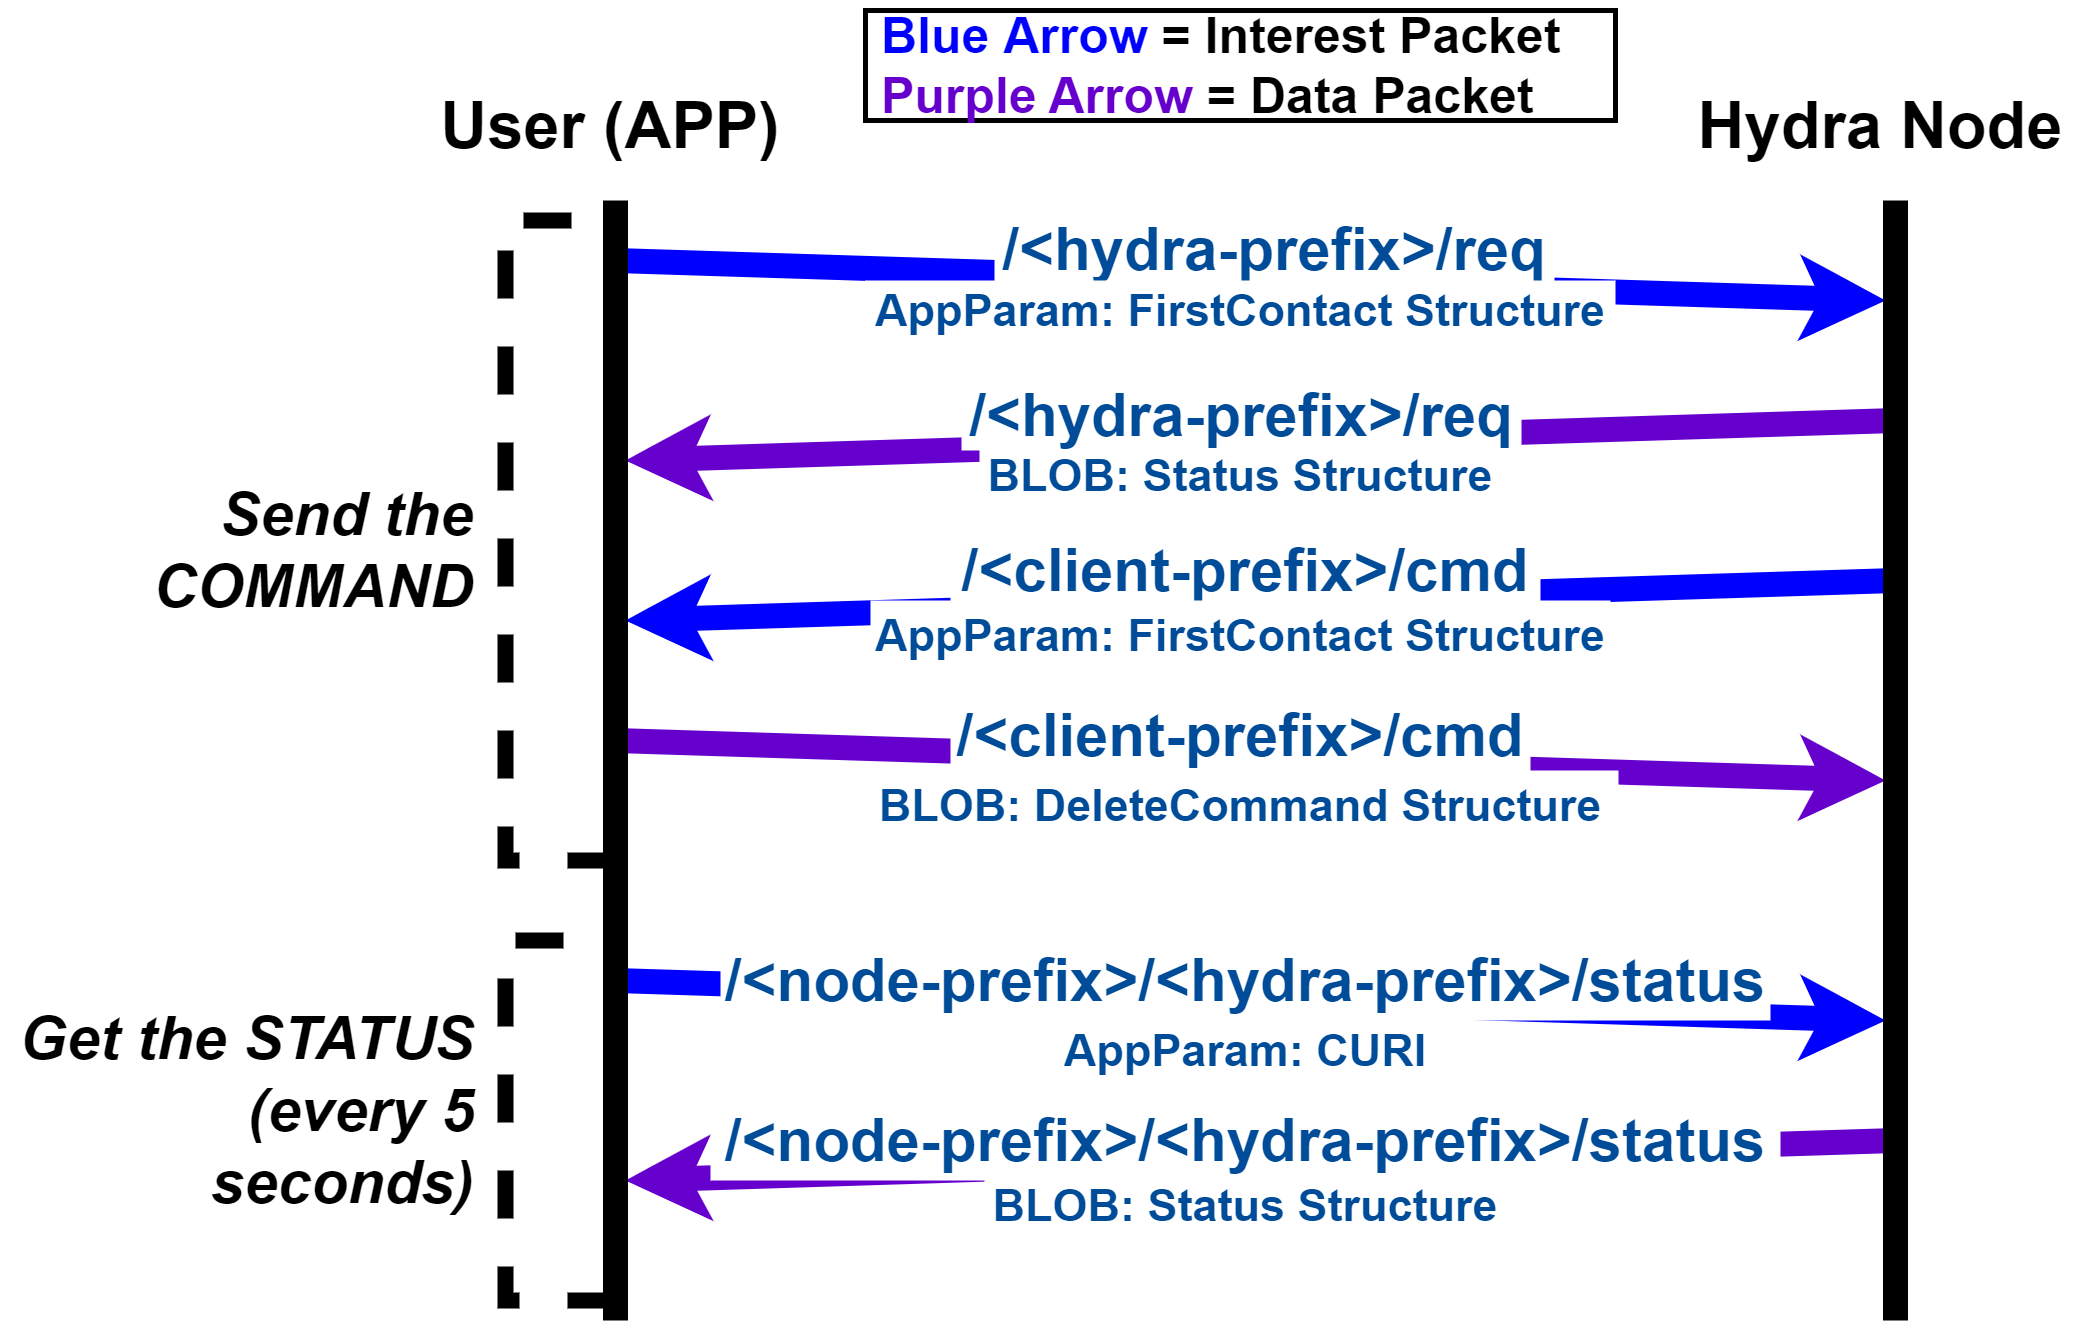
\includegraphics[width=\columnwidth]{visuals/delete-usr.png}
    \caption{NDN Interaction of a User and a Hydra Node During Deletion}
    \label{fig:delete-usr}
\end{figure}

The process of how a user will interact with a Hydra node via NDN is described in Figure~\ref{fig:delete-usr} and shares great similarities with data insertion. Any Hydra node can be contacted by the user for data deletion, and this interaction can be summarized as a PubSub-like interaction: it uses a notification interest with a component /notify and a data retrieval interest with a component /msg.

This interaction between user (A) and node (X) goes as follows:
\begin{enumerate}
    \item User (A) will send a interest notification using the prefix /<hydra-prefix/delete, announcing that it has a command for any Hydra node to process.
    \item Upon hearing this, node (X) will send an interest to fetch this command using user (A)'s prefix (stated in user (A)'s FirstContact structure found in the interest notification's app parameters).
    \item Node (X) will process this command and than send a notification interest stating that the command that user (A) sent has a updated status.
    \item User (A) can then fetch the status of the command using node (X)'s prefix (stated in node (X)'s FirstContact structure found in a previous interest).
\end{enumerate}

The exact same key points found in Subsection~\ref{sec:data-insert} for User-to-Node interaction applies for this process as well.


\subsubsection{Module Interaction} 
\begin{figure}[!ht]
    \centering
    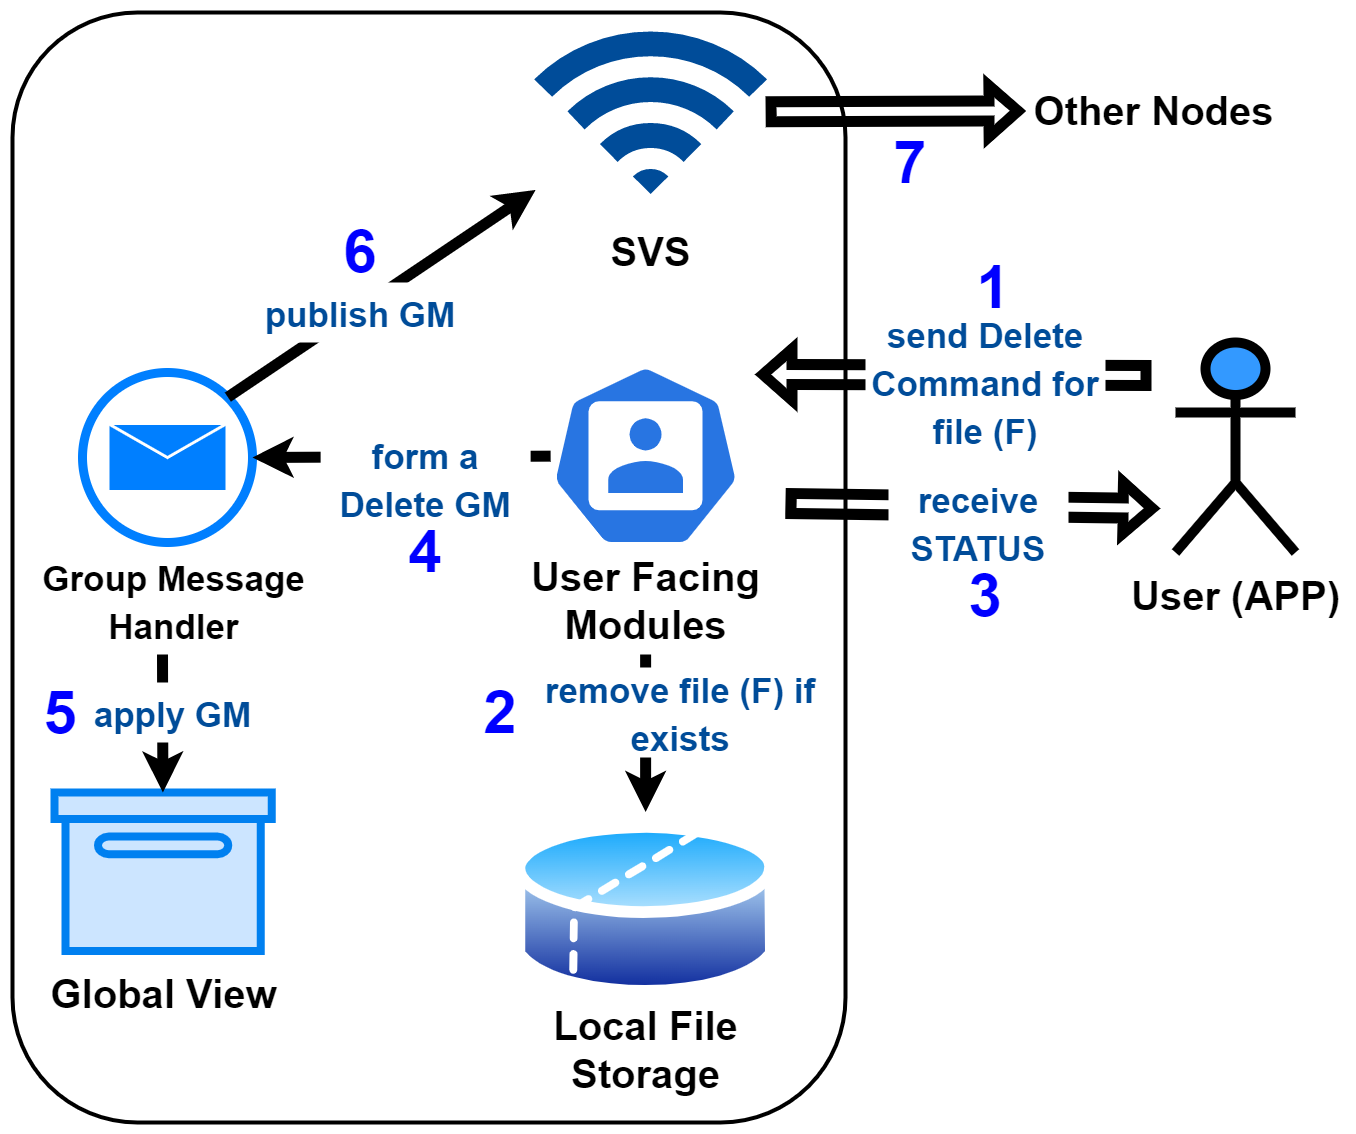
\includegraphics[width=\columnwidth]{visuals/delete-sys.png}
    \caption{Module Interaction to Fulfill a User's Deletion Command}
    \label{fig:delete-sys}
\end{figure}

The User-to-Node interaction leads to Module interaction where a Hydra node will act out the given command. As seen in Figure~\ref{fig:delete-sys}, when node (X) receives a Deletion command for file (F) from user (A):
\begin{enumerate}
    \item Node (X) properly authenticates the command.
    \item Node (X) deletes any local copies of file (F).
    \item Node (X) updates the status for user (A) allowing user (A) to go offline.
    \item Node (X) forms a Delete GM which includes the name of file (F).
    \item Node (X) applies this GM to its Global View: all file (F) information is removed.
    \item Node (X) publishes this GM using SVS, our distributed synchronization protocol.
\end{enumerate}

Every node will receive the Delete GM. When node (Y) receives the Delete GM sent by node (X) containing file (F)'s name:
\begin{enumerate}
    \item Node (Y) deletes any local copies of file (F).
    \item Node (Y) applies the GM to its Global View: all file (F) information is removed.
\end{enumerate}


\subsubsection{Data Structure Formats} 
There are several structures that are used for the entire data deletion process. For the group message structures used in Module interaction, please refer back to Section~\ref{sec:group-messages}. In addition, most of the other structures are the same ones described in Subsection~\ref{sec:data-insert}. The only missing structure is DeleteCommand which holds the filename of the desired-to-be-removed file.